\documentclass[12pt,openany]{book}
%\usepackage{classnotestikz}
%\usepackage{tikzelements}
\usepackage{libro-fciencias}
\usepackage{booktabs}
\usepackage{colortbl}
\def\thickline{\specialrule{.15em}{.05em}{.05em}}
\def\violetrule{\color{Violeta}{\rule{100px}{0.05em}}}
\def\bluerule{\color{DarkBlue}{\rule{100px}{0.05em}}}
\usepackage{multirow}


\usepackage{diagramas-fciencias}
\pgfplotsset{compat=1.15}

\graphicspath{ {Figuras/} }

%\setcounter{tocdepth}{4}

\addbibresource{rnnotesref.bib}


%----------------------------------------------------------------------------------------
%	Autores y Título
%----------------------------------------------------------------------------------------

\title{Redes Neuronales}
\subtitle{Notas de clase}
\author{Karla Fernanda Jiménez Gutiérrez\newline
        Verónica Esther Arriola Ríos}
\publisher{Facultad de Ciencias, UNAM}
\background{Neurona.png}


\begin{document}
\maketitle

%----------------------------------------------------------------------------------------
% Contenido
%----------------------------------------------------------------------------------------
\frontmatter % Numeración romana
\tableofcontents
\clearemptydoublepage % Whitespace to the end of the page


%----------------------------------------------------------------------------------------
%	                                Inicio
%----------------------------------------------------------------------------------------
\mainmatter  % Numeración arabiga


%%
\chapter*{Etc}

A lo largo del texto se utilizará la siguiente notación para diversos elementos:
\begin{longtable}{lc}
 Conjuntos   &   $\set{C}$ \\
 Vectores    &   $\vec{X}$ \\
 Matrices    &   $\mat{M}$ \\
 Unidades    &   $\unit{cm}$
\end{longtable}



%%
\part{Introducción}
\chapter{Historia de IA}
\section{Problemas representativos}
\subsection{Problema del marco}

\section{Agentes}


%%
\part{Resolución de problemas mediante búsqueda}
\chapter{Espacio de estados}
%\input{secciones/EspacioDeEstados}
\section{Espacio de estados continuo en física}
\section{Espacio de estados discreto}
\section{Mundo de juguete}

\chapter{Búsqueda}
\section{Búsqueda ciega}

\section{Problemas de satisfacción de restricciones}

\subsection{Definición}

\begin{definition}
Un problema de satisfacción de restricciones está definido por:
 \begin{itemize}
  \item Un conjunto de variables $\set{V} = \{X_1,X_2,...,X_n\}$
  \item Un conjunto de restricciones $\set{C} = \{C_1,C_2,...,C_m\}$
  \item Cada variable tiene un dominio asociado $\mathbb{D}_v$ con $\mathbb{D}_v \neq \emptyset$
 \end{itemize}
\end{definition}

Para este tipo de problemas 
\begin{itemize}
\item Un estado es una asignación a unas o todas las variables $\set{S} = \{X_i = v_i, X_j=v_j,...\}$
\item Una \emph{asignación consistente} es una asignación que no viola ninguna restricción.
\item Una \emph{asignación completa} es una asignación que menciona a todas las variables.
\item Una solución es una asignación completa y consistente.
\end{itemize}

Entonces el sistema de transiciones en el espacio de estados $\Sigma=(\set{S},\set{A},\gamma)$, queda definido con los elementos siguientes:
\begin{itemize}
 \item $\set{S}= \{s_1,s_2,...\}$ el conjunto de todas las posibles asignaciones (parciales y completas) a las variables del problema.
 \item $\set{A}= \{a_1,a_2,...\}$ el conjunto de las acciones que asignan a alguna variable $X_i$ un valor $v$ del dominio $\mathbb{D}_{X_i}$.
 \item $\gamma: S \times A \rightarrow S$ la función que aplica la acción $a_i$ en el estado $s_j$, si al realizar la asignación $a_i$, $s_j$ no queda en un estado inconsistente.  Para todos los demás casos, devuelve $\emptyset$ y se dice que la acción no es aplicable.
\end{itemize}

De este modo, el problema de planeación $\mathcal{P} = (\Sigma, s_i,g)$ usa:
  
\begin{itemize}
  \item $s_i = \{\}$ la asignación vacía.
  \item $g(s)$ la función que verifica si la asignación es completa.
\end{itemize}




\subsection{Recorrido en el espacio de búsqueda}

Para mostrar cómo se realiza una búsqueda en este espacio se utilizará el problema del \textit{Sudoku}.  Utilicemos como ejemplo el tablero mostrado en la \fref{fig:sudoku_vacio}.

\begin{figure}
 \centering
 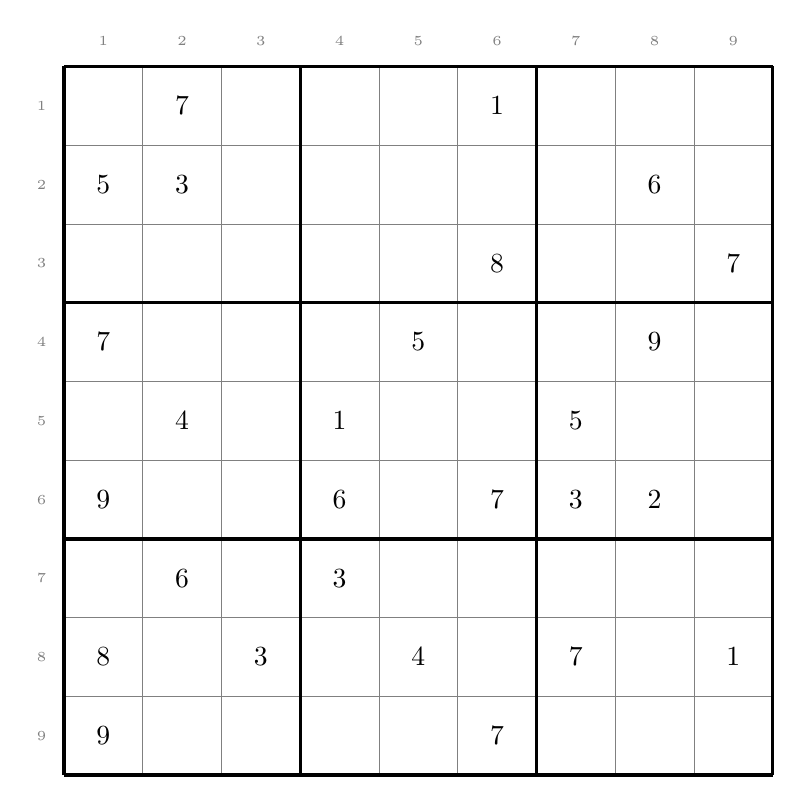
\begin{tikzpicture}
  \draw[step=1cm,gray,very thin] (0,0) grid (9,9);
  \draw[step=3cm,black,very thick] (0,0) grid (9,9);
  
  \node at (0.5cm,0.5cm) {9};
  \node at (5.5cm,0.5cm) {7};
  
  \node at (0.5cm,1.5cm) {8};
  \node at (2.5cm,1.5cm) {3};
  \node at (4.5cm,1.5cm) {4};
  \node at (6.5cm,1.5cm) {7};
  \node at (8.5cm,1.5cm) {1};
  
  \node at (1.5cm,2.5cm) {6};
  \node at (3.5cm,2.5cm) {3};
  
  \node at (0.5cm,3.5cm) {9};
  \node at (3.5cm,3.5cm) {6};
  \node at (5.5cm,3.5cm) {7};
  \node at (6.5cm,3.5cm) {3};
  \node at (7.5cm,3.5cm) {2};
  
  \node at (1.5cm,4.5cm) {4};
  \node at (3.5cm,4.5cm) {1};
  \node at (6.5cm,4.5cm) {5};

  \node at (0.5cm,5.5cm) {7};
  \node at (4.5cm,5.5cm) {5};
  \node at (7.5cm,5.5cm) {9};
  
  \node at (5.5cm,6.5cm) {8};
  \node at (8.5cm,6.5cm) {7};
  
  \node at (0.5cm,7.5cm) {5};
  \node at (1.5cm,7.5cm) {3};
  \node at (7.5cm,7.5cm) {6};
  
  \node at (1.5cm,8.5cm) {7};
  \node at (5.5cm,8.5cm) {1};
  
  \foreach \j in {1,...,9} { \node [anchor=north,gray] at (\j-0.5,9.5) {\tiny \j}; }
  \foreach \y [evaluate=\y as \i using int(10-\y)] in {1,...,9} { \node [anchor=east,gray] at (-0.1,\y-0.5) {\tiny \i}; }
 \end{tikzpicture}
 \caption{Tablero de Sudoku al iniciar un juego.}\label{fig:sudoku_vacio}
\end{figure}

En este escenario, las variables son las casillas vacías del Sudoku.  Sea $\set{X}$ el conjunto de todas las casillas.  Identifiquemos a cada casilla con el símbolo $X_{ij}$, con $i$ y $j$ en $\{1,2,...,9\}$, según su posición en el tablero.  Los valores posibles para cada casilla están en $\mathbb{D}_v = \{1,2,...,9\}$.

Dado que el juego del Sudoku comienza con valores en algunas casillas, el estado inicial ya tiene valores asociados a algunas de las $X_{ij}$.  Para el tablero del ejemplo se tendría la asignación inicial $F$:

\begin{align*}
 F = \{
 X_{12} =& 7,   &   X_{16} =& 1, \\
 X_{21} =& 5,   &   X_{22} =& 3,   &   X_{28} =& 6, \\
 ... \\
 X_{81} =& 8,   &   X_{83} =& 3,   &   X_{85} =& 4,   &   X_{87} =& 7,   &   X_{89} =& 1, \\
 X_{91} =& 9,   &   X_{96} =& 7\} \\
\end{align*}

Sin embargo, dado que los valores de estas casillas no pueden ser cambiados, este conjunto de casillas no pertenece al conjunto de variables.  Más bien se tiene:
\begin{align*}
 \set{V} = \set{X} - \set{F}
\end{align*}

Estimemos la complejidad inicial de este problema, calculando el número de estados posibles con asignaciones completas:
\begin{enumerate}
 \item Hay $|V|$ casillas vacías, cada una de las cuales puede albergar $9$ valores distintos.
 \item Esto da un total de $9^{|V|}$ asignaciones posibles.
\end{enumerate}
En el ejemplo anterior, son $9^{54} \approx 3.5\times10^{51}$.  Compárese con la capacidad de un disco duro de un terabyte, donde $1\unit{T} \approx 10^{12} \unit{bytes}$.  No intentemos siquiera agregar las asignaciones incompletas.  Claramente no es posible resolver este problema sin hacer uso de las restricciones, para evitar recorrer este espacio de estados.

\subsubsection{Propagación de restricciones}

Por la forma en que se planteó el problema en la sección anterior, se comienza la búsqueda de un solución, con la asignación vacía $s_i = \{\}$.  ¿Cuáles son las acciones aplicables en este momento?  Para comenzar: las acciones posibles son aquellas que asignan un valor a alguna de las casillas vacías.  Obsérvese que se estableció como precondición para su aplicabilidad, que el valor asignado no viole ninguna de las restricciones del problema.  En el caso del Sudoku, éstas son:
\begin{enumerate}
 \item Que no haya otra casilla en el mismo renglón, con el mismo valor.
 \item Que no haya otra casilla en la misma columna, con el mismo valor.
 \item Que no haya otra casilla en el mismo cuadrante, con el mismo valor.
\end{enumerate}

Consideremos ahora al conjunto $\mathbb{D}_v$ de valores posibles para cada variable.
Estas tres condiciones implican que, cada vez que se asigne un valor $v$, a una casilla $X_{ij}$, los valores que permiten una asignación consistente se reducen para las casillas siguientes:
\begin{enumerate}
 \item Todas las casillas en el renglón $i$, ya no pueden tener a $v$ como valor.
 \item Todas las casillas en la columna $j$, ya no pueden tener a $v$ como valor.
 \item Todas las casillas en el cuadrante $i$, ya no pueden tener a $v$ como valor.
\end{enumerate}

Antes de elegir la acción a aplicar, es necesario \emph{propagar} el efecto de estas restricciones, para determinar cuáles son las acciones aplicables en un estado dado.  Depués de hacer esto, quedarán grupos de acciones aplicables: un grupo por cada variable que aún no ha sido asignada, con tantas acciones asociadas, como valores sea posible asignarle.  Visualicemos esto como en la \fref{fig:sucesores_restricciones}.

\begin{figure}
 \centering
 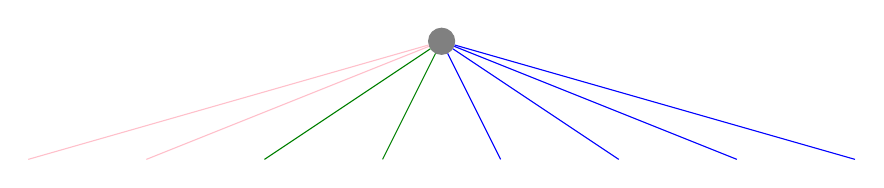
\begin{tikzpicture}
  \node [circle, fill=Gray, draw=Gray] {}
    child [circle, fill=Pink, draw=Pink] {}
    child [circle, fill=Pink, draw=Pink] {}
    child [circle, fill=Green, draw=Green] {}
    child [circle, fill=Green, draw=Green] {}
    child [circle, fill=Blue, draw=Blue] {}
    child [circle, fill=Blue, draw=Blue] {}
    child [circle, fill=Blue, draw=Blue] {}
    child [circle, fill=Blue, draw=Blue] {}
  ;
 \end{tikzpicture}
 \caption{Grupos de acciones aplicables y sus sucesores para un problema de satisfacción de restricciones.}\label{fig:sucesores_restricciones}
\end{figure}

Todas las variables que no han sido asignadas deberán recibir alguna asignación en algún momento.  Sin embargo, podemos seleccionar cual asignaremos primero y esto acelerará la búsqueda drásticamente.  También podemos elegir qué valor probaremos primero, de entre los que aún se le puede asignar.  Hay tres reglas que sugieren cómo realizar estas elecciones:


\section{Búsqueda informada: uso de heurísticas}
\subsection{Alpinismo de colinas}
\subsection{Recocido simulado}
\subsection{A*}

\section{Búsqueda con adversarios}
\subsection{Min-max}
\subsection{Poda \texorpdfstring{$\alpha-\beta$}{alfa-beta}}

\section{Sistemas de planeación}
\subsection{STRIPS, PDDL y CLIPS}
\subsubsection{Hipótesis del mundo cerrado}
\subsection{Planeación con órdenes parciales (PoP)}
\subsection{Redes de planeación jerárquica}
\subsection{Estados de creencia}
\subsection{Razonamiento no monótono (conocimiento incompleto)}

\chapter{Representación del conocimiento}
%%
%% Dibujos
%%
%\usepackage{tikz}
\usetikzlibrary{shapes,shapes.geometric,arrows,calc,fit,shadows,positioning,decorations.markings}
\tikzstyle{oval} = [ellipse, top color=white!70!Green!70, bottom color=Green, node distance=2cm, minimum height=2em, draw=Green]
\tikzstyle{arrow} = [->, decoration={markings,mark=at position 1 with {\arrow[scale=2]{>}}},
    postaction={decorate},
    shorten >=0.4pt]
\tikzstyle{marco} = [top color=white!70!AzulCielo!70, bottom color=AzulCielo, draw=AzulCielo]

% We need layers to draw the block diagram
\pgfdeclarelayer{background}
\pgfdeclarelayer{foreground}
\pgfsetlayers{background,main,foreground}


%opening
%\title{Marcos}
%\author{Inteligencia Artificial}

%\begin{document}

%\maketitle

\section{Marcos (Frames)}

El sistema de Marcos en la base de la programación Orientada a Objetos actual, por lo que los conceptos aquí citados resultarán familiares.  Sin embargo, la teoría de marcos cubre casos que la mayoría de los lenguades de programación populares evitan, especialmente la herencia múltiple.  Además, el término \textit{marco} en general puede referirse tanto a una instancia como a una clase \cite{Winston}.

Dos notaciones comunes para representar a los marcos son:
\begin{lstlisting}
 (nombre ranura(valor-de-ranura) ranura-1(valor-de-ranura-1)...)
\end{lstlisting}

\begin{figure}[H]
\centering
\begin{tikzpicture}
 \node (name) {Nombre};
 \node [label=west:slot, draw, below of=name, anchor=south west] (slot) {valor-de-ranura};
 \begin{pgfonlayer}{background}
  \node [marco, fit=(name)(slot), draw, inner sep=5pt, align=left] (marco) {};
 \end{pgfonlayer}
\end{tikzpicture}
\caption{Diagrama de un marco.}
\end{figure}

Los marcos se originaron a partir de las redes semánticas.  Una \textbf{red semántica} está compuesta por nodos y ligas entre ellos.  Cada liga lleva por nombre el tipo de relación entre los nodos vinculados.  Para reinterpretar una red semántica como un sistema de marcos se considera a cada nodo con las ligas vinculadas a él.

\begin{figure}[H]
\centering
\begin{tikzpicture}
 \node [oval] (manager) {Gerente};
 \node [oval, below of=manager] (grumpy) {Gruñón};
 \node [oval, right of=grumpy, node distance=10em] (happy) {Feliz};
 \draw [arrow] (grumpy) -- node [above] {le-agrada} (happy);
 \draw [arrow] (grumpy) -- node [right] {es-un} (manager);
 \draw [arrow] (manager) -- ($(manager) + (0,+1)$);
 \draw [arrow] (happy) -- ($(happy) + (+1,0)$);
 \draw [arrow] (happy) -- ($(happy) + (+1,+1)$);
\end{tikzpicture}
\\ \vspace{5mm}
\begin{tikzpicture}
 \node (name) {Gerentes};
 \node [label=west:, draw, below of=name, anchor=south west, text width=4em] (slot) {};
 \begin{pgfonlayer}{background}
  \node [marco, fit=(name)(slot), inner sep=5pt, align=left] (marco) {};
 \end{pgfonlayer}

 \node [below of=name, node distance=7em] (grumpy) {Gruñón};
 \node [label=west:is-a, draw, below of=grumpy, anchor=south west, text width=4em] (gEs_un) {};
 \node [label=west:le-agrada, draw, below of=gEs_un, anchor=south west, text width=4em] (gLikes) {Feliz};
 \begin{pgfonlayer}{background}
  \node [marco, fit=(grumpy)(gEs_un)(gLikes), draw, inner sep=5pt, align=left] (marco1) {};
 \end{pgfonlayer}
 \draw [*->] (gEs_un.center) -- +(0,1.7) -- +(-2.8,1.7) -- +(-2.8,2.7) -- (manager.west);

 \node [right of=grumpy, node distance=10em] (happy) {Feliz};
 \node [label=west:, draw, below of=happy, anchor=south west, text width=4em] (hEs_un) {};
 \node [label=west:, draw, below of=hEs_un, anchor=south west, text width=4em] (hLikes) {};
 \begin{pgfonlayer}{background}
  \node [marco, fit=(happy)(hEs_un)(hLikes), draw, inner sep=5pt, align=left] (marco2) {};
 \end{pgfonlayer}
\end{tikzpicture}
\caption{Arriba: red semántica.  Abajo: diagrama de un marco; es posible usar ligas o nombres de otros marcos para llenar las ranuras.}
\end{figure}

Hay dos clases de marcos:
\begin{itemize}
 \item Clases. a.k.o. = \emph{a kind of} <class>
 \item Ejemplares (o instancias). is-a <class>
\end{itemize}

\subsection{Procedimientos de acceso}
\begin{description}
 \item[Durante-la-construcción] construye marcos instancia.  Puede asignar valores por defecto a las ranuras mediante los \textbf{procedimientos-de-construcción} sugeridos por las clases y superclases de la instancia, de acuerdo con la \textbf{lista-de-precedencia}.
 \item[Durante-la-escritura] Asigna valores a las rendijas.  Ayudan a mantener restricciones entre ranuras relacionadas.  Por ejemplo: si en la ranura \textit{constitución-física} se escribe \textit{delgado}, escribir \textit{pequeño} en la ranura \textit{apetito}.
 \item[Durante-la-lectura] Devuelve los valores de las rendijas.
 \item[Cuando-se-solicite] Sobrecargan los valores por defecto heredados.  Pueden utilzar valores de otras ranuras que fueron llenadas durante la construcción de la instancia.
 \item[Con-respecto-a] reciben como argumento el contexto en el que la propiedad debe ser evaluada.  Por ejemplo, si se pide la estatura del enano Blimpy con repecto a un duente, el valor es \textit{grande}.  Si se pide su estatura con respecto a un enano promedio, tal vez el valor se \textit{pequeño}.
 \item[Cuando-aplica] semejante a los procedimientos \textit{con-respecto-a}, pero para acciones.  Calculan el mecanismo adecuado para cada acción dependiendo del contexto.  Por ejemplo: \texttt{comer(sopa)} utiliza una cuchara, mientras que \texttt{comer(ensalda)} require un tenedor.
\end{description}

\subsection{Lista de precedencia}
Hay dos criterios útiles para la obtención de una lista de precedencia:
\begin{enumerate}
 \item Cada clase debe aparecer en la lista de precedencia antes que cualquiera de sus superclases.
 \item Cada superclase directa de una clase dada debe aparecer en la lista de precedencia antes que cualquier superclase directa que se encuentre a su derecha.
\end{enumerate}

Si el tipo de herencia es simple, basta con recorrer la gráfica de marco primero en profundidad.  Si la herencia es múltiple, pero no se forman rombos en la jerarquía, basta con agregar la regla \textbf{up-to-join-proviso}.  Esta regla indica que, cada superclase que sea visitada más de una vez durante el recorrido primero en profundidad, de izquierda a derecha, debe ser ignorada hasta que la clase se encontrada por última vez.  Sin embargo, para el caso general, es necesario aplicar el algoritmo \textbf{ordenamiento topológico} [\pref{alg:topological_sort}].

% \begin{algorithm}[htp!]
%  \caption{Ordenamiento topológico.}\label{alg:astar}
% \begin{algorithmic}
%  \State listaMarcos $\leftarrow$ Crear una lista de todos los marcos accesibles desde el nodo instancia a través de relaciones is-a y a.k.o, incluyendo al nodo instancia.
%  \ForAll{marco \textbf{in} listaMarcos}
%    \If{marco.is-a $\neq\emptyset$}
%      \State listaRestricciones.add(marco, marco.is-a[0])
%      \ForAll{i,clase \textbf{in} marco.is-a[1:-1]}
%       \State listaRestricciones.add(clase, marco.is-a[i+1])
%      \EndFor
%    \EndIf
%    \If{marco.ako $\neq\emptyset$}
%      \State listaRestricciones.add(marco, clase.ako[0])
%      \ForAll{i,clase \textbf{in} clase.ako[1:-1]}
%       \State listaRestricciones.add(clase, clase.ako[i+1])
%      \EndFor
%    \EndIf
%  \EndFor
%  \ForAll{pair in listaRestricciones}
%   \If{pair.left \notin }
%  \EndFor
% \end{algorithmic}
% \end{algorithm}

\begin{algorithm}[H]
 \caption{Ordenamiento topológico.}\label{alg:topological_sort}
\begin{algorithmic}
 \State listaMarcos $\leftarrow$ Crear una lista de todos los marcos accesibles desde el nodo instancia a través de relaciones is-a y a.k.o, incluyendo al nodo instancia.
 \ForAll{marco \textbf{in} listaMarcos}
  \State listaRestricciones.añadir(marco, primer clase a la izquierda)
  \State Añadir listaRestricciones cada par clase-clase de izquierda a derecha
  \State Si el marco no tiene clases o superclases añadirlo solo.  Un elemento solo cuenta como estar a la izquierda del par.
 \EndFor
 \Repeat
 \State Tomar al marco que aparezca a la izquierda de al menos un par, pero a la deracha de ninguno.
  \If{Hay más de un marco sólo a la izquierda}
   \State Recorrer la listaDePresedencia desde el final hacia el inicio.
   \State Seleccionar el marco que sea clase o superclase directa del elemento más cercano al final de la listaDePresedencia.
  \EndIf
  \State Añadirlo a listaDePresedencia
  \State Eliminar a todos los pares donde aparezca.
 \Until{listaRestricciones $=\emptyset$}
\end{algorithmic}
\end{algorithm}

\begin{figure}
 \centering
 %\includegraphics[width=\textwidth]{../Figuras/Marcos.png}
  \caption{Objetos y relaciones diversas entre ellos.  Particularmente: \emph{un-tipo-de}, \emph{es-un} que permiten heredar comportamientos.}
\end{figure}


\subsection{Aplicaciones}
Extracción de información de textos en un contexto definido, así como producción de textos a partir de instancias con información.
Almacenamiento de información para sistemas expertos como:
\begin{itemize}
 \item CYC (\hurl{http://www.cyc.com/} y \hurl{http://www.cyc.com/platform/opencyc})
 \item OpenMind Common Sense \hurl{http://commons.media.mit.edu/}
\end{itemize}

Existe también una base datos del idioma Inglés donde las palabras están relacionadas unas con otras:
\begin{itemize}
 \item WordNet \hurl{http://wordnet.princeton.edu/}
\end{itemize}
 
%\end{document}
Otros


%%
\part{Aprendizaje de máquina}
\chapter{Aprendizaje automático}
\section{Tipos de aprendizaje}

\begin{description}
 \item [Aprendizaje supervisado] Aprender a predecir la salida, dado un vector de entrada.
 \begin{description}
  \item [Regresión] La salida está en $\mathbb{R}^n$.
  \item [Clasificación] La salida es discreta, usualmente etiquetas de clases.
 \end{description}
 
 \item [Aprendizaje no supervisado] Descubrir una buena representación para las entradas.  Una buena representación tiene las características siguientes:
 \begin{enumerate}
  \item Es compacta, es una representación en pocas dimensiones de entradas en varias dimensiones.
  \item Permite utilizar características que se pueden representar en forma económica (poco espacio).
 \end{enumerate}
 \begin{description}
  \item [Clasificación]
  \item [Análisis de componentes principales]
 \end{description}
 
 \item [Aprendizaje reforzado] Aprender a elegir una acción para maximizar una ganancia.
\end{description}
\section{Sesgo inductivo}
\section{Conjuntos de entrenamiento, prueba y validación}

\section{Regresión polinomial}
\subsection{Mínimos cuadrados}
\subsection{Forma normal}
\subsection{Descenso por el gradiente}
\subsection{Regularización}

\section{Clasificación}
\subsection{Regresión logística}
\subsection{Regularización}

\section{Redes neuronales}
\subsection{Perceptrón}
\subsection{Compuertas lógicas}
\subsection{Evaluación: Propagación hacia adelante}
\subsection{Entrenamiento: Propagación hacia atrás}

\section{Puff}
\section{Aprendizaje por refuerzo}
\section{K-medias}


%%
\part{Razonamiento Bayesiano}

\chapter{Antecedentes de probabilidad}

\section{Definiciones iniciales}

Un \emph{experimento causal, indeterminista o de azar} es aquel para el cual no necesariamente podemos predecir con certeza lo que va a ocurrir al realizarlo.  Cuando se repite el mismo experimento bajo las mismas condiciones se puede obtener un resultado diferente.
\begin{quotation}
 Ej: ``predecir el resultado de lanzar dos monedas.''
\end{quotation}

\begin{description}
 \item [Evento simple.] Cualquier resultado elemental de un experimento aleatorio.
  \begin{quotation}
   Ej: a: ``obtener el 2 al lanzar un dado.''
  \end{quotation}
  
 \item [Evento.] Cualquier conjunto de resultados posibles de un experimento aleatorio.
  \begin{quotation}
   Ej: A: ``obtener un par al lanzar un dado.''
   
       $A = \{2,4,6\} = \{$ ``obtengo el dos'', ``o... cuatro'', ``o... seis''$\} = \{x|x=2,4,6\}$
  \end{quotation}
  
 \item [Espacio de eventos, muestras o Universo $S$.]  Conjunto de todos los eventos simples posibles en un experimento aleatorio.
  \begin{quotation}
   Ej: ``lanzar un dado.''
   
       $S = \{1,2,3,4,5,6\}$
  \end{quotation}
 \item [Tamaño de un evento.] Número de eventos simples que satifacen la definición del evento (cardinalidad del conjunto).
 \begin{quotation}
  Ej: tamaño de A: $|A| = 3$.
 \end{quotation}
\end{description}

\begin{definition}
Definimos a la probabilidad de un evento $A$ como:
\begin{align}
 P(A) =& \dfrac{|A|}{|S|}. \label{eq:proba_laplace}
\end{align}

Destaca también lo que se conoce como la \emph{definición frecuentista} de probabilidad, en la cual esta cantidad $P(A)$ se define con respecto a una secuencia potencialmente infinita de repeticiones del experimento aleatorio $A$.
\end{definition}

Es posible representar gráficamente a los eventos utilizando \emph{diagramas de Venn}.  Por ejemplo, sea $S$ el Universo y $A$ un evento, su diagrama correspondiente se muestra en la \fref{fig:venn_a}.

\begin{figure}
  \centering
  \def\firstcircle{(0,0) circle (1.5cm)}
  \def\universesquare{(-3,-2) rectangle (3,2)}
  \begin{tikzpicture}
      \begin{scope}[fill opacity=0.5]
	  \fill[red] \firstcircle;
	  \draw \firstcircle [opacity=1] node {$A$};
	  \draw \universesquare [opacity=1] node [below left] {$S$};
      \end{scope}
  \end{tikzpicture}
  \caption{Evento $A$ en el espacio de eventos $S$.}\label{fig:venn_a}
\end{figure}

Se dice que dos eventos son \emph{mutuamente exclusivos} si no pueden ser verdad al mismo tiempo y se pueden visualizar como dos conjuntos ajenos \fref{fig:exclusivos}.

\begin{figure}
  \centering
  \def\firstcircle{(-1.25,0) circle (1cm)}
  \def\secondcircle{(1.25,0) circle (1cm)}
  \def\universesquare{(-3,-2) rectangle (3,2)}
  \begin{tikzpicture}
      \begin{scope}[fill opacity=0.5]
	  \fill[red] \firstcircle;
	  \draw \firstcircle [opacity=1] node {$A$};
	  \fill[red] \secondcircle;
	  \draw \secondcircle [opacity=1] node {$B$};
	  \draw \universesquare [opacity=1] node [below left] {$S$};
      \end{scope}
  \end{tikzpicture}
  \caption{Eventos mutuamente exclusivos $A$ y $B$ en el espacio de eventos $S$.}\label{fig:exclusivos}
\end{figure}

Eventos posibles incluyen al universo $S$ y al conjunto que no contiene resultados $\phi$.  Dados dos eventos $E$ y $F$ es posible crear otros eventos mediante las operaciones:

\begin{figure}
  \centering
  \def\firstcircle{(0,0) circle (1.5cm)}
  \def\secondcircle{(0:2cm) circle (1.5cm)}
  \def\universesquare{(-2,-2) rectangle (4,2)}
  \def\universesmall{(-2,-2) rectangle (2,2)}
  \begin{tikzpicture}
      \begin{scope}[fill opacity=0.5]
	  \fill[red] \firstcircle;
	  \fill[red] \secondcircle;
	  \draw \firstcircle [opacity=1] node [left] {$A$};
	  \draw \secondcircle [opacity=1] node [right] {$B$};
	  \draw \universesquare [opacity=1] node [below left] {$S$};
      \end{scope}
  \end{tikzpicture}
  \begin{tikzpicture}
      \begin{scope}[fill opacity=0.5]
	\begin{scope}
	  \clip \firstcircle;
	  \fill[red] \secondcircle;
	\end{scope}
	  \draw \firstcircle [opacity=1] node [left] {$A$};
	  \draw \secondcircle [opacity=1] node [right] {$B$};
	  \draw \universesquare [opacity=1] node [below left] {$S$};
      \end{scope}
  \end{tikzpicture}
  
  \vspace{2mm}
  \begin{tikzpicture}
      \begin{scope}[fill opacity=0.5]
	  \fill[red] \universesmall;
	  \fill[white, opacity=1] \firstcircle;
	  \draw \firstcircle [opacity=1] node {$A$};
	  \draw \universesmall [opacity=1] node [below left] {$S$};
      \end{scope}
  \end{tikzpicture}
  \caption{Arriba izquierda: Unión de eventos.  Arriba derecha: Intersección.  Abajo: Complemento.}\label{fig:creacionEventos}
\end{figure}

\begin{description}
 \item [Unión.] La unión de dos eventos $E \cup F$ es el conjunto de eventos simples en $E$ o $F$ inclusivamente. \fref{fig:creacionEventos} (Izquierda).
 \item [Intersección.]  La intersección de dos eventos $E \cap F$ es el conjunto de eventos simples en ambos $E$ y $F$ al mismo tiempo. \fref{fig:creacionEventos} (Derecha).
 \item [Complemento.] El complemento de un evento es el conjunto de los eventos simples que no se encuentran en $E$, denotado $\bar{E}$.
\end{description}



\section{Variable aleatoria}

Una variable aleatoria es una función que va del espacio de muestras a los reales $X : S \rightarrow \mathbb{R}$\footnote{Por convensión, escribiremos las variables aleatorias con mayúsculas y sus valores concretos con minúsculas.}.  Esta función permite medir el aspecto de interés para un evento dado, en función de los resultados elementales obtenidos. 
  \begin{quotation}
   Ej: Para el evento E:``obtener un 7 al lanzar dos dados''.
   
       Sea la variable aleatoria $X$ : ``La suma del resultado en cada uno de dos dados''.
   
       $X(dado_1, dado_2) = dado_1 + dado_2$
       
       Entonces el evento $E$ se expresa como $E : X(dado_1, dado_2) = 7$.
  \end{quotation}
Obsérvese que la función de la variable aleatoria puede ser, como un caso particular, la función identidad si el espacio de eventos está contenido en los reales.  Otro caso particular sería una función que realice un mapeo uno a uno del espacio de eventos hacia los reales.  Para ello es necesario que los valores en el dominio sean:
 \begin{enumerate}
  \item Mutuamente exclusivos.
  \item Exhaustivos.
 \end{enumerate}

 \begin{quotation}
  Ej: Formalmente la variable aleatoria $C(Clima)$ tendría el rango:
  \begin{align*}
   C(Clima) = <1, 2, 3, 4, 5>
  \end{align*}
 
  Dichos valores podrían venir de un mapeo directo con los valores del espacio de eventos:
   \begin{align*}
    Clima =& <despejado, lluvioso, nublado, granizado, nevado> \\
    C(Clima) =& \begin{cases}
		1	& \text{si } despejado \\
		2       & \text{si } lluvioso \\
		3	& \text{si } nublado \\
		4	& \text{si } granizado \\
		5	& \text{si } nevado
	      \end{cases}
   \end{align*}
   
   Esto también se puede escribir $C \in \{c^1,c^2,c^3,c^4,c^5\}$, que abrevia los casos $C=1,C=2,C=3,C=4,C=5$.
 \end{quotation}

 
De este modo es posible asociar una variable aleatoria a cada variable natural del espacio de eventos.  Por comodidad y legibilidad, frecuentemente se hará referencia a la variable del espacio de eventos como una \textit{variable aleatoria}, con un dominio diferente a los reales, aunque formalmente debe sobre-entenderse la existencia de un mapeo entre los elementos del espacio de eventos y los número reales.

\subsection{Variables aleatorias discretas y continuas}

Es posible clasificar a las variables aleatorias de acuerdo a las características de su rango en:
\begin{description}
 \item [Discretas.] Su rango consiste en un número finito de valores.
 
 Un caso particular de variables discretas son las variables booleanas, donde los valores que pueden tomar son $\{0,1\}$.
 
 Es posible asignar una probabilidad a cada valor de una variable aleatoria discreta, definiendo lo que será entonces una \emph{distribución de probabilidad}.  Dado que los valores de la variable aleatoria son exclusivos, la suma de las probabilidades sobre todos los valores debe ser $1$.

 \begin{quotation}
  Ej:
  \begin{align*}
   P(Clima) =&  \begin{cases}
		0.4	& \text{si } despejado \\
		0.25       & \text{si } lluvioso \\
		0.15	& \text{si } nublado \\
		0.1	& \text{si } granizado \\
		0.1	& \text{si } nevado
	      \end{cases}
  \end{align*}

 \end{quotation}
 
 \item [Continuas.] Al realizar un experimento aleatorio todos los valores sobre $\mathbb{R}$ o un intervalo $[a,b] \in \mathbb{R}$ son resultados posibles.
 \begin{quotation}
  Ej: ``$Temperatura \in [0,60000]\degree K$''.
 \end{quotation}
  Dado que el número de elementos en un intervalo continuo es infinito, la probabilidad de obtener un valor específico es cero.  Por consiguiente se define una \emph{función de densidad de probabilidad}\footnote{Obsérvese que, en principio, $f(x)$ puede tomar valores mayores que uno \cite{Barber2012}.}
  \begin{align}
   f(x) &\geq 0
  \end{align}
  a partir de la cual se calcula la probabilidad de que $X$ tome algún valor dentro de un subconjunto mesurable $B \in \mathbb{R}$ de sus valores posibles:
  \begin{align}
   P(X \in B) &= \int_B f(x) dx
  \end{align}
  En particular, si $B$ es un intervalo de $\mathbb{R}$ entonces:
  \begin{align}
   P(a \leq X \leq b) = \int_a^b f(x) dx
  \end{align}
  Dado que $X$ debe tomar algún valor en $\mathbb{R}$, entonces $P(X)$ debe satisfacer:
  \begin{align}
   P(X \in (-\infty,\infty)) = \int_{-\infty}^{\infty} f(x) dx = 1
  \end{align}
\end{description}

\subsection{Extensión de la lógica proposicional}
 
Es posible utilizar la teoría de probabilidades para extender a la lógica proposicional.  El tipo más sencillo de proposición a utilizar es la afirmación de que una variable aleatoria tiene un valor particular tomado de su dominio.
\begin{quotation}
 Ej: ``$Temperatura = 310$''.
\end{quotation}
Dicho esto, es posible asociar una probabilidad al evento de que una proposición dada sea verdadera o falsa.  Gracias a ello será posible realizar inferencias en condiciones de incertidumbre.


\section{Axiomas de la probabilidad}

Andrei Kolmogorov demostró cómo desarrollar el resto de la teoría probabilista a partir de los tres axiomas que llevan su nombre\footnote{\cite{Russell2004}}:

\begin{enumerate}
 \item Todas las probabilidades están entre 0 y 1. Para cualquier proposición $a$,
 \begin{equation}
  0 \leq P(a)\leq 1
 \end{equation}
 
 \item Las proposiciones necesariamente ciertas (es decir, válidas) tienen probabilidad 1, y las proposiciones necesariamente falsas (es decir, insatisfacibles) tienen probabilidad 0.
 \begin{align}
  P(cierto) =& 1 & P(falso) =& 0
 \end{align}
 
 \item La probabilidad de una disyunción viene dada por
 \begin{equation}
  P(a \lor b) = P(a) + P(b) - P(a \land b)
 \end{equation}
\end{enumerate}

\begin{figure}
  \centering
  \def\firstcircle{(0,0) circle (1.5cm)}
  \def\secondcircle{(0:2cm) circle (1.5cm)}
  \def\universesquare{(-2,-2) rectangle (4,2)}
  \begin{tikzpicture}
      \begin{scope}[fill opacity=0.5]
	  \fill[red] \firstcircle;
	  \fill[red] \secondcircle;
	  \draw \firstcircle [opacity=1] node [left] {$A$};
	  \draw \secondcircle [opacity=1] node [right] {$B$};
	  \draw \universesquare [opacity=1] node [below left] {$S$};
      \end{scope}
  \end{tikzpicture}
  \caption{La probabilidad $P(a \lor b)$ corresponde a la probabilidad de la unión de ambos eventos.}\label{fig:p_or}
\end{figure}

Este último axioma es fácilmente interpretable utilizando teoría de conjuntos \fref{fig:p_or}, pues utilizando la \eref{eq:proba_laplace} se tiene:

\begin{align*}
 P(a \lor b) = \dfrac{|a \cup b|}{|S|} = \dfrac{|a| + |b| - |a \cap b|}{|S|} = P(a) + P(b) - P(a \land b).
\end{align*}



\section{Probabilidad condicional}

\begin{figure}
  \centering
  \def\firstcircle{(0,0) circle (1.5cm)}
  \def\secondcircle{(0:2cm) circle (1.5cm)}
  \def\universesquare{(-2,-2) rectangle (4,2)}
  \begin{tikzpicture}
      \begin{scope}[fill opacity=0.5]
        \fill[gray] \secondcircle;
	\begin{scope}
	  \clip \firstcircle;
	  \fill[red] \secondcircle;
	\end{scope}
	  \draw \firstcircle [opacity=1] node [left] {$A$};
	  \draw \secondcircle [opacity=1] node [right] {$B$};
	  \draw \universesquare [opacity=1] node [below left] {$S$};
      \end{scope}
  \end{tikzpicture}
  \caption{La probabilidad $P(a | b)$ corresponde a la probabilidad de la intersección de ambos eventos, como si $B$ fuera el nuevo universo.}\label{fig:p_cond}
\end{figure}

Es posible definir la probabilidad de un evento sujeto a la evidencia observada como (\fref{fig:p_cond}):
\begin{align}
 P(a|b) = \dfrac{P(a \land b)}{P(b)} \label{eq:p_cond}
\end{align}

\section{Teorema de Bayes}

Si tomamos las definiciones de probabilidad condicional:
\begin{align}
 P(a|b) &= \dfrac{P(a \land b)}{P(b)} & P(b|a) &= \dfrac{P(a \land b)}{P(a)}
\end{align}
y despejamos la probabilidad conjunta en ambas expresiones:
\begin{align}
 P(a \land b) = P(b) P(a|b) = P(a) P(b|a)
\end{align}
obtenemos la fórmula del \emph{teorema de Bayes}:
\begin{align}
 P(b|a) = \frac{P(a|b)P(b)}{P(a)}
\end{align}

\subsection{A priori, a posteriori y verosimilitud}

Asociada al teorema de Bayes existe una terminología particuar.  La misma fórmula puede ser reescrita como sigue:
\begin{align}
 p(\theta | e ) = \dfrac{p(e | \theta) p(\theta)}{p(e)}
\end{align}
donde a $p(\theta)$ se le conoce como la \emph{creencia a priori} \footnote{\textit{Prior} en inglés} de que ocurra $\theta$.  Esta variable puede representar cualquier cosa, por ejemplo una enfermedad como la varicela o el sarampeon.  La característica especial de esta variable es que suele corresponder a algo que no podemos saber directamente si ocurrió o no.  Lo único que podemos hacer es inferir la probabilidad de que haya ocurrido, dependiendo de la presencia una cierta evidencia $e$ que sí podemos medir (por ejemplo la presencia de manchas rojas en la piel).  Usualmente para obtener un diagnóstico, necesitaríamos la probabilidad $p(\theta | e)$ de que haya ocurrido $\theta$ dependiendo del valor de la evidencia $e$; como esta probabilidad se obtiene posteriormente a la presentación de la evidencia, se le suele conocer como \emph{a posteriori} \footnote{\textit{Posterior} en inglés.}.

Desafortunadamente, es más fácil modelar $p(e | \theta)$, la probabilidad de que se presente la evidencia, dada su causa.  A esta probabilidad se le conoce como \emph{verosimilitud}\footnote{\textit{Likelihood} en inglés.}.

A $p(e)$ no quisieron darle nombre porque representa a la probabilidad de que la evidencia se presente, en general y hay quienes la concideran \textit{sólo una constante de normalización}, aunque no por ello deja de ser relevante.  A menudo es frecuente encontrar la fórmula expresada como:
\begin{align}
 p(\theta | e ) \propto p(e | \theta) p(\theta)
\end{align}



\section{Distribuciones de probabilidad}

Una \emph{distribución de probabilidad} asocia a cada valor posible de una variable aleatoria la probabilidad de que se obtenga ese valor al realizar un experimento.  Por ejemplo:

\begin{center}
\begin{tabular}{c|c}
 $Lluvia$ & $P(Lluvia)$ \\ \toprule
 0 & 0.6375 \\
 1 & 0.3625 \\
 \multicolumn{1}{c}{}  & $\sum=1$
\end{tabular}
\end{center}

Una \emph{distribución de probabilidad conjunta} asocia a cada combinación posible de los valores de varias variables que se revisan simulatáneamente, la probabilidad de que se obtenga esa combinación al realizar un experimento.  Por ejemplo:

\begin{center}
\begin{tabular}{cc|c}
 $Estaci\acute{o}n$ & $Lluvia$ & $P(Lluvia \land Estaci\acute{o}n)$ \\ \toprule
 Primavera & 0 & 0.1875 \\
 Primavera & 1 & 0.0625 \\
 Verano & 0 & 0.075 \\
 Verano & 1 & 0.175 \\
 Otoño & 0 & 0.175 \\
 Otoño & 1 & 0.075 \\
 Invierno & 0 & 0.2 \\
 Invierno & 1 & 0.05 \\
 \multicolumn{2}{c}{}  & $\sum=1$
\end{tabular}
\end{center}

De esta tabla se pueden leer directamente respuestras a preguntas como ``¿Cuál es la probabilidad de que sea primavera y llueva?'', donde la respuesta sería $0.0625$.

Si las variables siendo consideradas, son todas las variables del sistema, entonces se dice que se tiene la \emph{distribución de probabilidad conjunta completa}.

La \emph{distribución de probabilidad condicional} asocia una probabilidad a cada combinación de valores de variables, dado un valor determinado para un conjunto de variables evidencia.  Por ejemplo: ¿cuál es la probabilidad de que llueva, sabiendo la estación del año? Un ejemplo concreto extraído de esta tabla sería ``¿Cuál es la probabilidad de que llueva, si es primavera?'' y la respuesta es $0.25$.

\begin{center}
\begin{tabular}{c|cccc}
 $Lluvia$ / $Estaci\acute{o}n$ & Primavera & Verano & Otoño & Invierno \\ \toprule
 0 & 0.75 & 0.30 & 0.70 & 0.80 \\
 1 & 0.25 & 0.70 & 0.30 & 0.20 \\
 \multicolumn{1}{c}{}  & $\sum=1$ & $\sum=1$ & $\sum=1$ & $\sum=1$
\end{tabular}
\end{center}


\section{La regla de la cadena}

Así como se definió a la probabilidad condicional en términos de una probabilidad conjunta y la probabilidad de la variable evidencia en \eref{eq:p_cond}, es posible generalizar la definición a varias variables.
Para simplificar la notación a partir de este momento, en lugar de utilizar el tradicional símbolo $\land$ para denotar la relación $y$ o $intersecci\acute{o}n$, indicaremos a la probabilidad conjunta separando a las variables con comas.  De este modo la ecuación citada se convierte en:
\begin{align}
 P(a|b) = \dfrac{P(a \land b)}{P(b)} = \dfrac{P(a, b)}{P(b)}
\end{align}
de donde habíamos despejado:
\begin{align}
 P(a, b) &= P(a|b)P(b)
\end{align}


Cuando queremos expresar a la probabilidad de obtener la conjunción de varias variables, dada la conjunción de otra variables, la fórmula se verá como:
\begin{align}
 P(X_1,X_2,...,X_n|Y_1,Y_2,...,Y_n) = \dfrac{P(X_1,X_2,...,X_n,Y_1,Y_2,...,Y_n)}{P(Y_1,Y_2,...,Y_n)}
\end{align}
de donde despejamos:
\begin{align}
 P(X_1,X_2,...,X_n,Y_1,Y_2,...,Y_n) = P(X_1,X_2,...,X_n|Y_1,Y_2,...,Y_n)P(Y_1,Y_2,...,Y_n)
\end{align}
En particular, si comenzamos por condicionar a la primera variable con respecto a las demás en la conjunción, se verá así:
\begin{align}
 P(X_1,X_2,...,X_n) = P(X_1|X_2,...,X_n)P(X_2,...,X_n)
\end{align}
repitiendo el mismo proceso con los términos como $P(X_2,...,X_n)$ obtenemos la fórmula conocida como \emph{regla de la cadena}:

\begin{align}
 P(X_1,X_2,...,X_n) = P(X_1|X_2,...,X_n)P(X_2|X_3,...,X_n)...P(X_n)
\end{align}


\section{Compuertas lógicas con probabilidades}

Para iniciar con el uso de probabilidades para inferencia lógica, comenzaremos por ilustrar cómo la inferencia exacta puede ser vista como un caso particular de la inferencia con probabilidades, mediante la definición de la compuertas lógicas $or$ y $and$ en términos de probabilidades.  Se dejará como un ejercicio para el lector definir a la compuerta $or$.

Para esto se definirán distribuciones de probabilidad condicional: la salida de la compuerta lógica, condicionada al valor de las entradas.  Asignando probabilidad uno a las combinaciones correctas de variables de entrada/salida y cero a las opciones inválidas.

\begin{center}
%\begin{box}
  \begin{tabular}{cc|c} \hline
   \multicolumn{3}{c}{\emph{No}: $\lnot$} \\ \hline
   $x$ & $y$ & $P(y|x)$ \\ \hline
   0 & 0 & 0 \\
   0 & 1 & 1 \\
   1 & 0 & 1 \\
   1 & 1 & 0 \\ \hline
  \end{tabular}
  \hspace*{1cm}%
  \begin{tabular}{ccc|c} \hline
   \multicolumn{4}{c}{\emph{Y}: $\land$} \\ \hline
   $x_1$ & $x_2$ & $y$ & $P(y|x_1,x_2)$ \\ \hline
   0 & 0 & 0 & 1 \\
   0 & 0 & 1 & 0 \\
   0 & 1 & 0 & 1 \\
   0 & 1 & 1 & 0 \\
   1 & 0 & 0 & 1 \\
   1 & 0 & 1 & 0 \\
   1 & 1 & 0 & 0 \\
   1 & 1 & 1 & 1 \\ \hline
  \end{tabular}
%\end{box}
\end{center}

Ganamos la posibilidad de modelar compuertas ruidosas, que no siempre devuelven la respuesta correcta, asociando una pequeña probabilidad $\varepsilon \neq 0$ a las respuestas incorrectas y ajustando acordemente las correctas:

\begin{center}
%\begin{box}
  \begin{tabular}{cc|c} \hline
   \multicolumn{3}{c}{\emph{No}: $\lnot$} \\ \hline
   $x$ & $y$ & $P(y|x)$ \\ \hline
   0 & 0 & $\varepsilon$ \\
   0 & 1 & $1 - \varepsilon$ \\
   1 & 0 & $1 - \varepsilon$ \\
   1 & 1 & $\varepsilon$ \\ \hline
  \end{tabular}
  \hspace*{1cm}%
  \begin{tabular}{ccc|c} \hline
   \multicolumn{4}{c}{\emph{Y}: $\land$} \\ \hline
   $x_1$ & $x_2$ & $y$ & $P(y|x_1,x_2)$ \\ \hline
   0 & 0 & 0 & $1 - \varepsilon$ \\
   0 & 0 & 1 & $\varepsilon$ \\
   0 & 1 & 0 & $1 - \varepsilon$ \\
   0 & 1 & 1 & $\varepsilon$ \\
   1 & 0 & 0 & $1 - \varepsilon$ \\
   1 & 0 & 1 & $\varepsilon$ \\
   1 & 1 & 0 & $\varepsilon$ \\
   1 & 1 & 1 & $1 - \varepsilon$ \\ \hline
  \end{tabular}
%\end{box}
\end{center}

\chapter{Factores}

\begin{definition}[Factor]
Un factor $\phi(X_1,...,X_k)$, sobre variables $X_i$, donde cada $X_i$ puede tomar valores de un dominio $D_{X_i}$ es una función:

\begin{align}
 \phi : Val(X_1,...,X_k) \rightarrow \mathbb{R}
\end{align}
que asocia un número real a posibles asignaciones de valores a las variables $X_1,...,X_k$.  El \emph{alcance} $\mathbb{A}$ de un factor son las variables cuyos posibles valores están siendo considerados.
\begin{align}
 \mathbb{A}(\phi(X_1,...,X_k)) = \{X_1,...,X_k\}
\end{align}
\end{definition}


\begin{example}
Un factor.  Sean las variables y dominios:
\begin{itemize}
 \item $Estaci\acute{o}n$, $D_{Estaci\acute{o}n}=\{Primavera, Verano, Oto\tilde{n}o,Invierno\}$
 
 \item $Lluvia$, $D_{Lluvia}=\{0,1\}$
\end{itemize}
de modo que el alcance es $\mathbb{A} = \{Estaci\acute{o}n, Lluvia\}$

\begin{center}
\rowcolors{2}{\colTableRow}{white}
\begin{tabular}{cc|c}
 $Estaci\acute{o}n$ & $Lluvia$ & Frecuencia (días/mes) \\ \hline
 Primavera & 0 & 18 \\
 Primavera & 1 & 6 \\
 Verano & 0 & 7 \\
 Verano & 1 & 17 \\
 Otoño & 0 & 17 \\
 Otoño & 1 & 7 \\
 Invierno & 0 & 20 \\
 Invierno & 1 & 5 \\
\end{tabular}
\end{center}
\end{example}


Se utilizarán factores para representar las distribuciones de probabilidad, distribuciones de probabilidad conjuntas y condicionales.

\section{Marginalización}

\begin{definition}[Marginalización]
Dada una variable $X_i$, en el alcance $\mathbb{A}$ de un factor $\phi = \phi(X_1,...,X_k)$, que se desea marginalizar, se define a la operación como:
\begin{align}
 marginalizaci\acute{o}n(\phi(X_1,...,X_k), X_i) =& \phi'(\mathbb{A'}) \\
 \mathbb{A'} =& \mathbb{A}(\phi) - X_i \text{ con } i \in [1,k] \\
 \phi'(x_1,...,x_{i-1},x_{i+1},...,x_k) =& \sum_{Val\{X_i\}} \phi(x_1,...,x_k)
\end{align}
donde $x_i$ es un valor particular de $X_i$, $\phi'(x_1,...,x_{i-1},x_{i+1},...,x_k)$ es el renglón del factor $\phi'$ con $\{X_1 = x_i,..., X_k=x_k\}$ y $Val\{X_i\}$ es el conjunto de valores posibles asignables a $X_i$.
\end{definition}

\begin{example}{Marginalizar $Estaci\acute{o}n$}
\begin{center}
\rowcolors{2}{\colTableRow}{white}
\begin{tabular}{cc|c}
 $Estaci\acute{o}n$ & $Lluvia$ & $P(Lluvia,Estaci\acute{o}n)$ \\ \toprule
 Primavera & 0 & 0.1875 \\
 Primavera & 1 & 0.0625 \\
 Verano & 0 & 0.075 \\
 Verano & 1 & 0.175 \\
 Otoño & 0 & 0.175 \\
 Otoño & 1 & 0.075 \\
 Invierno & 0 & 0.2 \\
 Invierno & 1 & 0.05 \\
 \multicolumn{2}{c}{}  & $\sum=1$
\end{tabular}$\Rightarrow$\rowcolors{2}{\colTableRow}{white}
\begin{tabular}{c|c}
 $Lluvia$ & $P(Lluvia)$ \\ \toprule
 0 & 0.63750 \\
 1 & 0.36250 \\
 \multicolumn{1}{c}{}  & $\sum=1$
\end{tabular}
\end{center}
\end{example}


\section{Reducción}

\begin{definition}[Reducción]
Dado un valor $x_i = a$ para una de las variables $X_i$ en el alcance $\mathbb{A}$ del factor $\phi$, se reduce el factor eliminando todas aquellas entradas en las cuales no se cumple que $X_i = a$.  La operación se define como:
\begin{align}
 reducci\acute{o}n(\phi(X_1,...,X_k), X_i, a) =& \phi'(\mathbb{A'}) \\
 \mathbb{A'} =& \mathbb{A}(\phi) - X_i \text{ con } i \in [1,k] \\
 \phi'(x_1,...,x_{i-1},x_{i+1},...,x_k) =& \phi(x_1,...,x_k) \text{ con } X_i = a
\end{align}
\end{definition}

A diferencia de las distribuciones de probabilidad, la reducción en un factor no requiere renormalizar sus valores asociados, pues por definición, no es necesario que éstos sumen uno.

\begin{example}{Reducir $Estaci\acute{o}n = Primavera$}
\begin{center}
\begin{tabular}{cc|c}
 $Estaci\acute{o}n$ & $Lluvia$ & $P(Lluvia,Estaci\acute{o}n)$ \\ \toprule
 \rowcolor{\colTableRow} Primavera & 0 & 0.1875 \\
 \rowcolor{\colTableRow} Primavera & 1 & 0.0625 \\
 Verano & 0 & 0.075 \\
 Verano & 1 & 0.175 \\
 Otoño & 0 & 0.175 \\
 Otoño & 1 & 0.075 \\
 Invierno & 0 & 0.2 \\
 Invierno & 1 & 0.05 \\
 \multicolumn{2}{c}{}  & $\sum=1$
\end{tabular}$\Rightarrow$
\begin{tabular}{c|c}
 $Lluvia$ & $P(Lluvia,Estaci\acute{o}n = primavera)$ \\ \toprule
 0 & 0.1875 \\
 1 & 0.0625 \\
 \multicolumn{1}{c}{}  & $\sum=0.25$
\end{tabular}
\end{center}
\end{example}


\section{Normalización}

\begin{definition}[Normalización]
Dado un factor $\phi$ con $n$ renglones sea
\begin{align}
 s =& \sum_{i=1}^n \phi_i
\end{align}
con $\phi_i$ el valor asociado al renglón $i$, $s$ es la suma de los valores de todos los renglones.  Entonces:
\begin{align}
 normalizaci\acute{o}n(\phi) =& \phi' \\
 \phi'_i = \dfrac{\phi_i}{s}
\end{align}
donde el valor en cada renglón de $\phi$ ha sido dividido entre $s$.
\end{definition}

\begin{example}{Normalizar}
\begin{center}
\begin{tabular}{c|c}
 $Lluvia$ & $P(Lluvia,primavera)$ \\ \toprule
 0 & 0.1875 / 0.25 \\
 1 & 0.0625 / 0.25 \\
 \multicolumn{1}{c}{}  & $\sum=0.25$
\end{tabular}$\Rightarrow$
\begin{tabular}{c|c}
 $Lluvia$ & $P(Lluvia|primavera)$ \\ \toprule
 0 & 0.75 \\
 1 & 0.25 \\
 \multicolumn{1}{c}{}  & $\sum=1$
\end{tabular}
\end{center}
\end{example}


\section{Multiplicación}

\begin{definition}[Multiplicación]
Se define el producto de factores de tal modo que:
\begin{align}
 \phi_1 =& \phi_1(X_1,...,X_k) \\
 \phi_2 =& \phi_2(Y_1,...,Y_l) \\
 \phi =& \phi_1 \phi_2 \\
 \mathbb{A}(\phi) =& \mathbb{A}(\phi_1) \cup \mathbb{A}(\phi_2) \\
 \phi(z_1,...,z_m) =& \phi_1(x_1,...,x_k) * \phi_2(y_1,...,y_l)
\end{align}
donde $Z_k \in \mathbb{A}(\phi)$ por lo que:
\begin{align}
 \text{ si } Z_k \in \mathbb{A}(\phi_1) & \Rightarrow Z_k = X_i \land z_k = x_i \\
 \text{ si } Z_k \in \mathbb{A}(\phi_2) & \Rightarrow Z_k = Y_j \land z_k = y_j
\end{align}
obsérvese que si $Z_k \in \mathbb{A}(\phi_1)$ y $Z_k \in \mathbb{A}(\phi_2)$ entonces $Z_k = X_i = Y_j$ y en cada renglón deberá cumplirse $z_k = x_i = y_j$.
\end{definition}


\begin{example}{Multiplicar $P(Lluvia|Estaci\acute{o}n)P(Estaci\acute{o}n)$}
\begin{center}
\begin{tabular}{cc|c}
 $Estaci\acute{o}n$ & $Lluvia$ & $P(Lluvia|Estaci\acute{o}n)$ \\ \toprule
 \rowcolor{\colTableRow}Primavera & 0 & 0.75 \\
 \rowcolor{\colTableRow}Primavera & 1 & 0.25 \\
 \rowcolor{\colTableRowOne}Verano & 0 & 0.30 \\
 \rowcolor{\colTableRowOne}Verano & 1 & 0.70 \\
 \rowcolor{\colTableRowTwo}Otoño & 0 & 0.70 \\
 \rowcolor{\colTableRowTwo}Otoño & 1 & 0.30 \\
 \rowcolor{\colTableRowThree}Invierno & 0 & 0.80 \\
 \rowcolor{\colTableRowThree}Invierno & 1 & 0.20
\end{tabular}$\times$
\begin{tabular}{c|c}
 $Estaci\acute{o}n$ & $P(Estaci\acute{o}n)$ \\ \toprule
 \rowcolor{\colTableRow}Primavera & 0.25 \\
 \rowcolor{\colTableRowOne}Verano & 0.25 \\
 \rowcolor{\colTableRowTwo}Otoño & 0.25 \\
 \rowcolor{\colTableRowThree}Invierno & 0.25 \\
 \multicolumn{1}{c}{}  & $\sum=1$
\end{tabular}$=$

\begin{center}
\begin{tabular}{cc|c}
 $Estaci\acute{o}n$ & $Lluvia$ & $P(Lluvia,Estaci\acute{o}n)$ \\ \toprule
 \rowcolor{\colTableRow}Primavera & 0 & 0.1875 \\
 \rowcolor{\colTableRow}Primavera & 1 & 0.0625 \\
 \rowcolor{\colTableRowOne}Verano & 0 & 0.075 \\
 \rowcolor{\colTableRowOne}Verano & 1 & 0.175 \\
 \rowcolor{\colTableRowTwo}Otoño & 0 & 0.175 \\
 \rowcolor{\colTableRowTwo}Otoño & 1 & 0.075 \\
 \rowcolor{\colTableRowThree}Invierno & 0 & 0.2 \\
 \rowcolor{\colTableRowThree}Invierno & 1 & 0.05 \\
 \multicolumn{2}{c}{}  & $\sum=1$
\end{tabular}
\end{center}
\end{center}
\end{example}


\begin{example}{Multiplicar $P(Lluvia)P(Estaci\acute{o}n)$}
\begin{center}
\begin{tabular}{c|c}
 $Lluvia$ & $P(Lluvia)$ \\ \toprule
 \rowcolor{gray!10}0 & 0.63750 \\
 1 & 0.36250 \\
 \multicolumn{1}{c}{}  & $\sum=1$
\end{tabular}
$\times$
\begin{tabular}{c|c}
 $Estaci\acute{o}n$ & $P(Estaci\acute{o}n)$ \\ \toprule
 \rowcolor{\colTableRow}Primavera & 0.25 \\
 \rowcolor{\colTableRowOne}Verano & 0.25 \\
 \rowcolor{\colTableRowTwo}Otoño & 0.25 \\
 \rowcolor{\colTableRowThree}Invierno & 0.25 \\
 \multicolumn{1}{c}{}  & $\sum=1$
\end{tabular}$=$

Sea $R = P(Lluvia)P(Estaci\acute{o}n)$

\begin{center}
\begin{tabular}{cc|c}
 $Estaci\acute{o}n$ & $Lluvia$ & $R$ \\ \toprule
 \rowcolor{\colTableRow}Primavera & 0 & 0.159375 \\
 \rowcolor{\colTableRow!30}Primavera & 1 & 0.090625 \\
 \rowcolor{\colTableRowOne}Verano & 0 & 0.159375 \\
 \rowcolor{\colTableRowOne!30}Verano & 1 & 0.090625 \\
 \rowcolor{\colTableRowTwo}Otoño & 0 & 0.159375 \\
 \rowcolor{\colTableRowTwo!30}Otoño & 1 & 0.090625 \\
 \rowcolor{\colTableRowThree}Invierno & 0 & 0.159375 \\
 \rowcolor{\colTableRowThree!30}Invierno & 1 & 0.090625 \\
 \multicolumn{2}{c}{}  & $\sum=1$
\end{tabular}$=$
\begin{tabular}{cc|c}
 $Estaci\acute{o}n$ & $Lluvia$ & $R$ \\ \toprule
 \rowcolor{\colTableRow}Primavera & 0 & 0.159375 \\
 \rowcolor{\colTableRowOne}Verano & 0 & 0.159375 \\
 \rowcolor{\colTableRowTwo}Otoño & 0 & 0.159375 \\
 \rowcolor{\colTableRowThree}Invierno & 0 & 0.159375 \\
 \rowcolor{\colTableRow!30}Primavera & 1 & 0.090625 \\
 \rowcolor{\colTableRowOne!30}Verano & 1 & 0.090625 \\
 \rowcolor{\colTableRowTwo!30}Otoño & 1 & 0.090625 \\
 \rowcolor{\colTableRowThree!30}Invierno & 1 & 0.090625 \\
 \multicolumn{2}{c}{}  & $\sum=1$
\end{tabular}
\end{center}
\end{center}
\end{example}


\section{Distribuciones de probabilidad con factores}

Claramente, los factores pueden contener, en particular, tablas de distribuciones de probabilidad sobre variables discretas.  Las variables aleatorias del sistema aparecerán en el alcance del factor, las combinaciones posibles de asignaciones a estas variables quedarán registradas en los renglones del factor y la probabilidad de que ocurran será el número real asociado a esa entrada.


\subsection{Distribuciones de probabilidad condicional con factores}

Para escribir la distribución de probabilidad condicional utilizando factores, la notación cambia un poco.  Por ejemplo:

\begin{center}
\begin{tabular}{cc|cc}
 $Estaci\acute{o}n$ & $Lluvia$ & $P(Lluvia|Estaci\acute{o}n)$ \\ \toprule
 Primavera & 0 & 0.75 & \multirow{2}{*}{$\sum=1$} \\
 Primavera & 1 & 0.25 \\ \arrayrulecolor{gray}\cline{1-3}
 Verano & 0 & 0.30 & \multirow{2}{*}{$\sum=1$} \\
 Verano & 1 & 0.60 \\ \arrayrulecolor{gray}\cline{1-3}
 Otoño & 0 & 0.70 & \multirow{2}{*}{$\sum=1$} \\
 Otoño & 1 & 0.30 \\ \arrayrulecolor{gray}\cline{1-3}
 Invierno & 0 & 0.8 & \multirow{2}{*}{$\sum=1$} \\
 Invierno & 1 & 0.1 \\
\end{tabular}
\end{center}

\chapter[Independencia]{Dependencia e independencia probabilística}

\section{Independencia}

Dos eventos $\alpha$ y $\beta$ son independientes $P \models \alpha \perp \beta$\footnote{Se lee: $P$ satisface que $\alpha$ es independiente de $\beta$.} si:

\begin{align}
 P(\alpha \cap \beta) =& P(\alpha)P(\beta) \\
 P(\alpha|\beta) =& P(\alpha) \\
 P(\beta|\alpha) =& P(\beta)
\end{align}

Se dice que dos variables aleatorias $A$ y $B$ son \emph{independientes} $P \models A \perp B$ si se cumple que:

\begin{align}
 P(A,B) =& P(A)P(B) \\
 P(A|B) =& P(A) \\
 P(B|A) =& P(B)
\end{align}

No hay forma de representar el concepto de independencia con diagramas de Venn.  Obsérvese que independencia y exclusión ($A \cap B = \emptyset$) son dos conceptos distintos.

\section{Independencia condicional}

Se dice que dos eventos/variables aleatorias $E_1$ y $E_2$ son \emph{condicionalmente independientes} dado $F$, $P \models (E_1 \perp E_2 | F)$ si, dado que $F$ ocurre, la probabilidad condicional de que $E_1$ ocurra no cambia al obtenerse información sobre si $E_2$ ocurre o no.  Esto se escribe:

\begin{align}
 P(E_1|E_2F) =& P(E_1|F) \\
 P(E_2|E_1F) =& P(E_2|F) \\
\end{align}
o equivalentemente:
\begin{align}
 P(E_1E_2|F) = P(E_1|F)P(E_2|F)
\end{align}

Ejemplo: Se tienen dos monedas, una cargada de modo que 90\% del tiempo el resultado de un volado con ella será sol y otra moneda normal $Moneda = <Cargada, Normal>$.  Se elige una moneda al azar y se lanzan dos volados $Volado_i=<Sol, \acute{A}guila>$ [\fref{fig:condicionalMoneda}].  Inicialmente conocer el resultado del primer volado brinda información sobre la posibilidad de haber elegido la moneda cargada y por ende acerda del posible resultado del siguiente volado.  Sin embargo, si se sabe qué moneda se eligió, esa información es suficiente para conocer la probabilidad de cada resultado en el segundo volado, la información del primer volado ya no es relevante.  En este caso se dice que el resultado del segundo volado es independiente del resultado del primero, dado que se sabe qué moneda fue elegida.

\begin{figure}
 \centering
 \begin{tikzpicture}[->,>=stealth',level/.style={sibling distance = 5cm/#1, level distance = 1.5cm}]
  \node [ellipse,violetNode]{$Moneda$} [level distance=10mm,sibling distance=25mm]
    child { node [ellipse,cobaltNode] {$Volado_1$} }
    child { node [ellipse,cobaltNode] {$Volado_2$} };
 \end{tikzpicture}
 \caption{Un ejemplo de independencia condicional.  El resultado de cada volado con una moneda depende de si se eligió una moneda normal o una moneda cargada.  Si se sabe qué moneda se eligió, conocer el resultado de un volado ya no dice nada nuevo sobre el resultado de otro volado con la misma moneda.}\label{fig:condicionalMoneda}
\end{figure}


\section{Redes Bayesianas}

\begin{definition}[Red Bayesiana]
 Una \emph{Red Bayesiana} es:
 \begin{itemize}
  \item Una gráfica acíclica dirigida (GDA) $G$ cuyos nodos representan a las variables aleatorias $X_1,...,X_n$.
  \item Para cada nodo $X_i$ define una distribución de probabilidad condicional
  \begin{align}
   P(X_i|Padres_G(X_i))
  \end{align}
 \end{itemize}
\end{definition}

La red de Bayes representa un distribución de probabilidad conjunta para la cual se cumple, debido a la relación de independencia condicional entre las variables, que:
\begin{align}
 P(X_1,...,X_n) = \prod_i P(X_i|Padres_G(X_i))
\end{align}
A esta fórmula se le conoce como regla de la cadena para Redes Bayesianas.  Cuando un distribución de probabilidad conjunta $P$ satisface esta relación, se dice que $P$ \emph{se factoriza sobre} $G$.

\subsection{Independencia en redes bayesianas}


\begin{definition}[Ruta]
 Una \emph{ruta} $X_1-...-X_k$ es una secuencia de nodos que se encuentran conectados entre sí mediante una sola arista (no dirigida) en la gráfica.
\end{definition}

\begin{figure}
\centering
\begin{tikzpicture}[->,>=stealth',level/.style={sibling distance = 5cm/#1, level distance = 1cm}]
 \node [ellipse, cobaltNode] (D) {$X_1$};
 \node [ellipse, cobaltNode, right= of D] (I) {$X_3$};
 \node [ellipse, cobaltNode, below right= 1cm and 0.3cm of D] (G) {$X_2$};
 \node [ellipse, cobaltNode, below right= 1cm and 0.3cm of I] (S) {$X_4$};
 \node [ellipse, cobaltNode, below= of G] (L) {$X_5$};
 \draw [arrow,draw=red] (D) -- (G);
 \draw [arrow,draw=black] (I) -- (G);
 \draw [arrow,draw=black] (I) -- (S);
 \draw [arrow,draw=red] (G) -- (L);
\end{tikzpicture}\hspace*{2cm}
\begin{tikzpicture}[->,>=stealth',level/.style={sibling distance = 5cm/#1, level distance = 1cm}]
 \node [ellipse, cobaltNode] (D) {$X_1$};
 \node [ellipse, cobaltNode, right= of D] (I) {$X_3$};
 \node [ellipse, violetNode, below right= 1cm and 0.3cm of D] (G) {$X_2$};
 \node [ellipse, cobaltNode, below right= 1cm and 0.3cm of I] (S) {$X_4$};
 \node [ellipse, cobaltNode, below= of G] (L) {$X_5$};
 \draw [arrow,draw=red] (D) -- (G);
 \draw [arrow,draw=red] (I) -- (G);
 \draw [arrow,draw=red] (I) -- (S);
 \draw [arrow,draw=black] (G) -- (L);
\end{tikzpicture}
\caption{Izquierda: Ruta activa $X_1-X_2-X_5$.  Derecha: Ruta $X_1-X_2-X_3-X_4$ con estructura-v entre $X_1-X_2-X_3$, activada porque $X_2$ fue observada.}\label{fig:rutas}
\end{figure}



\subsubsection{Ruta activa}

Sea $\mathbb{Z}$ el conjunto de variables evidencia cuyo valor ha sido observado.

\nocite{Koller2009}
\begin{definition}
\begin{itemize}
 \item  Una ruta se encuentra \emph{activa} si no tiene \emph{estructuras-v} (dos padres $X_{i-1},X_{i+1}$ de un nodo común $X_i$, $X_{i-1} \rightarrow X_{i} \leftarrow X_{i+1}$) [\fref{fig:rutas} (Izquierda)].
 
 \item Una ruta $X_1 - ... - X_k$ está \emph{activa dado $\mathbb{Z}$} si:
 \begin{itemize}
  \item Para cualquier \textit{estructura-v} $X_{i-1} \rightarrow X_i \leftarrow X_{i+1}$ se tiene que $X_i$ o alguno de sus descencientes están en $\mathbb{Z}$.
  \item Ningún otro $X_i$ está en $\mathbb{Z}$.
 \end{itemize}
\end{itemize}
\end{definition}


\begin{exercise}
 Dada la red Bayesiana en la \fref{fig:senderosActivos}, determinar si los senderos siguientes son activos, dado que la variable $G$ fue observada:\footnote{Ejericio tomado del curso en línea de Daphne Koller.}
 \begin{enumerate}
  \item $C \rightarrow D \rightarrow G \leftarrow I \rightarrow S$ \gtick
  \item $I \rightarrow G \rightarrow L \rightarrow J \rightarrow H$
  \item $I \rightarrow S \rightarrow J \rightarrow H$ \gtick
  \item $C \rightarrow D \rightarrow G \leftarrow I \rightarrow S \rightarrow J \leftarrow L$
 \end{enumerate}

\end{exercise}

\begin{figure}
\begin{center}
 \begin{tikzpicture}
  \node [oval] (C) {C};
  \node [oval, below of=C] (D) {D};
  \node [oval, cobaltNode, below right of=D] (G) {G};
  \node [oval, above right of=G] (I) {I};
  \node [oval, below of=G] (L) {L};
  \node [oval, below right of=I] (S) {S};
  \node [oval, below right of=L] (J) {J};
  \node [oval, below left of=L] (H) {H};
  \draw [-Stealth] (C) -- (D);
  \draw [-Stealth] (D) -- (G);
  \draw [-Stealth] (I) -- (G);
  \draw [-Stealth] (I) -- (S);
  \draw [-Stealth] (G) -- (L);
  \draw [-Stealth] (G) -- (H);
  \draw [-Stealth] (S) -- (J);
  \draw [-Stealth] (J) -- (H);
  \draw [-Stealth] (L) -- (J);
 \end{tikzpicture}
\end{center}
\caption{Ejemplo de gráfica de Bayes con $G$ observado.}\label{fig:senderosActivos}
\end{figure}

\subsubsection{D-separación}

\begin{definition}
 Dos variables aleatorias $X$ y $Y$ se encuentran \emph{d-separadas} en $G$ dado $\mathbb{Z}$ si no existe una ruta activa entre $X$ y $Y$ dado $\mathbb{Z}$.
 \begin{align}
  d-sep_G(X,Y|Z)
 \end{align}
\end{definition}

\begin{theorem}
 Si la distribución de probabilidad $P$ se factoriza sobre $G$ y $d-sep_G(X,Y|Z)$ entonces $P$ satisface $(X \perp Y | Z)$.
\end{theorem}

Cualquier nodo se encuentra $d-separado$ de sus no descendientes dados sus padres $\Rightarrow$ Si $P$ se factoriza sobre $G$, entonces en $P$ cualquier variable es independiente de sus no-descendientes dados sus padres.


\begin{example}
 Indique si existe una d-separación en los casos siguientes:
 \begin{enumerate}
  \item $d-sep(D,I|L)$
  \item $d-sep(D,J|L)$
  \item $d-sep(D,J|L,I)$ \gtick
  \item $d-sep(D,J|L,H,I)$
 \end{enumerate}

\end{example}

\begin{figure}
\begin{center}
 \begin{tikzpicture}
  \node [oval] (C) {C};
  \node [oval, below of=C] (D) {D};
  \node [oval, below right of=D] (G) {G};
  \node [oval, blackNode, above right of=G] (I) {I};
  \node [oval, cobaltNode, below of=G] (L) {L};
  \node [oval, below right of=I] (S) {S};
  \node [oval, below right of=L] (J) {J};
  \node [oval, greenNode, below left of=L] (H) {H};
  \draw [-Stealth] (C) -- (D);
  \draw [-Stealth] (D) -- (G);
  \draw [-Stealth] (I) -- (G);
  \draw [-Stealth] (I) -- (S);
  \draw [-Stealth] (G) -- (L);
  \draw [-Stealth] (G) -- (H);
  \draw [-Stealth] (S) -- (J);
  \draw [-Stealth] (J) -- (H);
  \draw [-Stealth] (L) -- (J);
 \end{tikzpicture}
\end{center}
\caption{Ejemplo de gráfica de Bayes con $I$, $L$ y $H$ observados. $I$ bloquea el flujo, $H$ lo habilita y $L$ varía su función dependiendo del sendero analizado.}\label{fig:senderosActivos1}
\end{figure}




\subsection{Mapas de independencias (Mapas-I)}

Si la distribución de probabilidades conjuntas $P$ satisface todas las relaciones de independencia $I$ implicadas por las $d-separaciones$ de una gráfica $G$ se dice que $G$ es un mapa de independencias de $P$.
\begin{align}
 I(G) = \{(X \perp Y | Z) : d-sep_G(X,Y|Z)\}
\end{align}
Los mapas de independencias para $P$ no son únicos y no necesariamente contienen todas las relaciones de independencia que son válidas en $P$.
Si $G$ es un mapa de independencias para $P$, entonces $P$ se factoriza sobre $G$, para demostrar esto se utiliza la regla de la cadena y el hecho de que cualquier nodo es independiente de sus no descendientes dados su padres.


\subsection{I-Equivalencia}

\begin{figure}
 \centering
 \begin{tikzpicture}[->,>=stealth']
  \node [ellipse, cobaltNode] (X) {$X$};
  \node [ellipse, cobaltNode, right = 5mm of X] (Y) {$Y$};
  \node [ellipse, cobaltNode, right = 5mm of Y] (Z) {$Z$};
  \draw (X) -- (Y);
  \draw (Y) -- (Z);
 \end{tikzpicture}
 \hspace*{1cm}
 \begin{tikzpicture}[->,>=stealth']
  \node [ellipse, cobaltNode] (X) {$X$};
  \node [ellipse, cobaltNode, right = 5mm of X] (Y) {$Y$};
  \node [ellipse, cobaltNode, right = 5mm of Y] (Z) {$Z$};
  \draw (Y) -- (X);
  \draw (Y) -- (Z);
 \end{tikzpicture}
 \hspace*{1cm}
 \begin{tikzpicture}[->,>=stealth']
  \node [ellipse, cobaltNode] (X) {$X$};
  \node [ellipse, cobaltNode, right = 5mm of X] (Y) {$Y$};
  \node [ellipse, cobaltNode, right = 5mm of Y] (Z) {$Z$};
  \draw (Y) -- (X);
  \draw (Z) -- (Y);
 \end{tikzpicture}
 
 \vspace*{1cm}
 \begin{tikzpicture}[->,>=stealth']
  \node [ellipse, cobaltNode] (X) {$X$};
  \node [ellipse, cobaltNode, right = 5mm of X] (Y) {$Y$};
  \node [ellipse, cobaltNode, right = 5mm of Y] (Z) {$Z$};
  \draw (X) -- (Y);
  \draw (Z) -- (Y);
 \end{tikzpicture}
 \caption{Arriba: Tres gráficas $I-equivalentes$.  Abajo: Gráfica no $I-Equivalente$ a las anteriores.}\label{fig:iequiv}
\end{figure}


Dos gráficas $G_1$ y $G_2$ sobre $X_1,...,X_n$ son $I-Equivalentes$ si los conjuntos de independencias derivadas de ambas gráficas son iguales \fref{fig:iequiv}.
\begin{align}
 I(G_1) = I(G_2)
\end{align}


\subsection{Inferencia}
\subsection{Eliminación de variables}
\subsection{Modelo Ingenuo de Bayes}

Es un modelo particular utilizado para problemas de clasificación, que asume que todas las características $C_i$ de una clase $Clase$ son independientes entre sí, dada información sobre la clase, esto es $\forall C_i,C_j(C_i \perp C_j|Clase)$ [\fref{fig:naiveBayes}], de tal modo que la factorización siguiente es válida:
\begin{align}
 P(Clase,C_1,...,C_n) = P(Clase) \prod^n_{i=1}P(C_i|Clase)
\end{align}


\begin{figure}
 \centering
 \begin{tikzpicture}[->,>=stealth',level/.style={sibling distance = 20mm/#1, level distance = 1.5cm}]
  \node [ellipse,violetNode]{$Clase$} [level distance=10mm,sibling distance=10mm]
    child { node [ellipse,cobaltNode] {$C_1$} }
    child { node [ellipse,cobaltNode] {$C_2$} }
    child { node {...} }
    child { node [ellipse,cobaltNode] {$C_n$} };
 \end{tikzpicture}
 \caption{En modelo Ingenuo de Bayes, las características de una clase son independientes, dada la clase.}\label{fig:naiveBayes}
\end{figure}



\subsection{Inferencia aproximada}
\subsubsection{Muestreo directo}
\subsubsection{Verosimilitud ponderada}
\subsubsection{Muestreo Montecarlo en cadenas de Makov (MCCM)}


\section{Redes Bayesianas Dinámicas}
{\color{red} Sección incompleta.}

Sea $X$ una variable aleatoria cuyo valor cambia con el tiempo.  La probabilidad de una secuencia de eventos que ocurren a tiempos discretos $t=\{0,...,T\}$ se expresa:
\begin{align*}
 P(X^{(0:T)}) = P(X^{(0)})\prod^{T-1}_{t=0}P(X^{(t+1)}|X^{(0:t)})
\end{align*}
utilizando la regla de la cadena.

La \emph{hipótesis de Márkov} asume que:
\begin{align}
 (X^{(t+1)} \perp X^{(0:t-1)}|X^{(t)})
\end{align}
entonces se cumple que:
\begin{align}
 P(X^{(0:T)}) = P(X^{(0)})\prod^{T-1}_{t=0}P(X^{(t+1)}|X^{(t)})
\end{align}

Otra simplificación que se puede hacer al modelo es asumir \emph{independencia temporal}, a lo cual también se le conoce como asumir que el sistema es \emph{estacionario}.  Esto se expresa:
\begin{align}
 P(X^{(t+1)}|X^{(t)}) &= P(X'|X) & \forall t
\end{align}
Es decir, la dinámica del sistema no cambia con el tiempo.

Un sistema puede estar descrito por un conjunto de variables para cada tiempo y las premisas de independecia se aplican sobre ellas.  Para aliviar las restricciones del modelo, estas variables pueden codificar información derivada de otras relaciones temporales.  Por ejemplo: en un problema de localización de un vehículo, se puede agregar a la velocidad como variable que describe el estado.

\cite{Ross2013, Bolstad2007}
%\bibliography{ianotesref}

%\end{document}



%\section{Definición de probabilidad}

\section{Inferencia en redes de Markov}

\subsection{Aprendizaje en redes Bayesianas}
\subsubsection{Máxima verosimilitud}
\subsubsection{Estimación Bayesiana}


%%
\part{Robótica Inteligente}
\chapter{Cierre: Inteligencia artificial y el cerebro}

%----------------------------------------------------------------------------------------
% Bibliografia
%----------------------------------------------------------------------------------------
\backmatter

\printbibliography[heading=bibintoc]

\end{document}
